\documentclass[tikz]{standalone}
\usepackage{pgfplots}
\pgfplotsset{compat=1.15}
\usepackage{mathrsfs}
\usetikzlibrary{arrows,calc}
\usepackage{tkz-euclide}

\usepackage{fp}
\pagestyle{empty}

\definecolor{AngleClr}{rgb}{0,0.39215686274509803,0}
\definecolor{ShapeClr}{rgb}{0.6,0.2,0}

\begin{document}

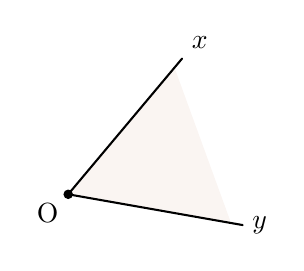
\begin{tikzpicture}[scale=.75]
\tkzSetUpLine[line width=1pt,color=black]
\tkzSetUpPoint[fill=black]

\tkzDefPoints{0/0/B}
\tkzDefPoint(50:3){A}
\tkzDefPoint(50:2.8){AA}
\tkzDefPoint(-10:3){C}
\tkzDefPoint(-10:2.8){CC}

\tkzFillPolygon[fill=ShapeClr,fill opacity=0.05](AA,B,CC)

\tkzDrawPoints[size=3](B)
\tkzLabelPoint[above right](A){$x$}
\tkzLabelPoint[below left](B){$\rm O$}
\tkzLabelPoint[right](C){$y$}

\tkzDrawSegments[line width=0.75pt](A,B B,C)

\end{tikzpicture}

\end{document}
